%% IEEE Transactions on Computers adaptation of the frozen FGCS manuscript.
%% The rejected FGCS source under ../Paper is preserved unchanged.
\documentclass[journal,10pt]{IEEEtran}

\usepackage{cite}
\usepackage[T1]{fontenc}
\usepackage{amsmath,amssymb,amsthm}
\usepackage{booktabs,multirow,array}
\usepackage{graphicx}
\usepackage{xcolor}
\usepackage{url}
\usepackage[hidelinks]{hyperref}
\usepackage{microtype}
\usepackage{stfloats}

\newtheorem{definition}{Definition}[section]
\newtheorem{theorem}{Theorem}[section]
\newtheorem{lemma}[theorem]{Lemma}
\newtheorem{corollary}[theorem]{Corollary}
\newtheorem{proposition}[theorem]{Proposition}
\newtheorem{assumption}[theorem]{Assumption}
\theoremstyle{remark}
\newtheorem{remark}[theorem]{Remark}

\newcommand{\state}{S}
\newcommand{\audio}{A}
\newcommand{\out}{Y}
\newcommand{\proj}{\Phi}
\newcommand{\ediv}{e}
\newcommand{\cont}{C}
\newcommand{\dist}{D}
\newcommand{\tx}{\tau}
\newcommand{\commit}{\Gamma}
\newcommand{\cert}{\mathrm{cert}}
\newcommand{\granratio}{\rho}
\newcommand{\tbl}[1]{\input{tables/#1}}
\newcommand{\artifactavailability}{A review artifact containing source code,
frozen audited results, and analysis scripts accompanies this submission; a
public archive will be released upon acceptance.}

\begin{document}

\title{RevTrace: A Transactional Runtime for Feedback-State Integrity in
Revision-Generative ASR Serving}

\author{Bin Zhou, Jiyuan Miao, and Xi Cao
\thanks{The authors are with Beijing University of Chemical Technology,
Beijing, China (e-mail: 2025200800@buct.edu.cn;
2024200822@buct.edu.cn; caoxi@buct.edu.cn).}
\thanks{Corresponding author: Xi Cao.}}

\markboth{IEEE Transactions on Computers, Submitted 2026}{}
\maketitle
\bstctlcite{IEEEexample:BSTcontrol}

\begin{abstract}
Revision-generative automatic speech recognition (ASR) pipelines feed model
outputs back into later execution
state. Under batched accelerator execution, a local numerical difference can
therefore become persistent state contamination. We formalize this failure mode
and introduce Dual-Granularity Feedback Transactions (DGFT), a runtime protocol
that separates low-latency proposal and display from canonical state-write
authority. Each accepted projection is bound to a certificate, parent version,
input frontier, and runtime configuration; same-granularity certification is
the $\granratio=1$ case. RevTrace implements DGFT as a two-plane parallel
runtime with independently replicated proposers and authorities. Across
Qwen3-ASR and Whisper on two RTX~3090 GPUs, coarse authority improves
matched-workload throughput by $1.39\times$/$1.28\times$ and reaches up to
$6.88\times$ wall-clock speedup over per-path all-singleton references, with
no observed installation violation in
800 Qwen events and 1{,}048 Whisper commits. A 250{,}000-attempt protocol
fuzzer rejects every mutation and replay. On eight V100 GPUs, balanced
replication sustains $157.8\times$/$111.7\times$ audio real-time throughput at
the largest measured concurrency satisfying the 2-s display service-level
objective (SLO). These results establish
state-write authorization as a distinct runtime contract for feedback-driven
ASR serving.
\end{abstract}

\begin{IEEEkeywords}
runtime systems, generative model serving, streaming ASR, state certification,
transactional consistency
\end{IEEEkeywords}

\section{Introduction}\label{sec:intro}
%% TC adaptation: runtime stake -> feedback-write failure -> mechanism -> evidence.

Accelerator-backed generative services usually treat a returned sequence as an
endpoint. Revision-generative ASR does not: Whisper-style decoders condition on
previously generated text~\cite{radford2023whisper,machacek2023whisperstreaming},
and Qwen3-ASR re-prompts itself with rollback prefixes from earlier
revisions~\cite{shi2026qwen3asr}. A generated hypothesis therefore mutates the
state of later execution. Yet throughput-oriented runtimes optimize request
scheduling and output delivery without exposing an authorization boundary
between model generation and this feedback write~\cite{kwon2023vllm,yu2022orca,zheng2024sglang}.

Batching improves accelerator utilization by sharing execution across
sessions~\cite{kwon2023vllm,agrawal2024sarathi,zhong2024distserve,sun2024llumnix},
but it can change floating-point reduction order and hence a greedy token
sequence relative to singleton execution~\cite{yuan2025numerical}. A terminal
service contains that difference within one response. In a revision-generative
service, the differing output can become the parent of every later revision
(Fig.~\ref{fig:motivation}). Controlled paired interventions establish that
this is a feedback-channel failure, not merely display variation: 8 of 21
legal state pairs propagate when the feedback edge is present, none propagate
when it is removed, and the measured revision amplification factor (RAF)
reaches 153.

Existing mechanisms regulate different boundaries. LocalAgreement stabilizes
display prefixes but does not authorize feedback parents~\cite{machacek2023whisperstreaming};
speculative decoding verifies draft tokens against a target
distribution~\cite{leviathan2023specdec,chen2023specsample}; and LLM-42 provides
verify--rollback for deterministic token generation, not revision-state
installation~\cite{zhang2026llm42}. Numerical reproducibility repairs execution
rather than state provenance~\cite{yuan2025numerical}. Optimistic concurrency
control supplies a useful analogy~\cite{kung1981occ,bernstein1983mvcc}, but here
the speculative write is a model-generated projection whose legality must be
established by the serving runtime.

We accordingly treat each revision output as a speculative state write:
$\mathrm{Display}(\out_t)\nRightarrow
\mathrm{Authorize}(\proj(\out_t;H_t))$. We introduce \textbf{Dual-Granularity
Feedback Transactions} (DGFT), which decouples a fine-grained proposal/display
path from a coarse canonical authority. Only a certificate bound to the parent
version, input frontier, projection, and execution contract can install state;
same-granularity certification is the $\granratio=1$ case. \textbf{RevTrace}
implements DGFT as a two-plane parallel runtime with contract-scoped
certification. The abstraction targets feedback-driven generation, while all
empirical generality claimed here is explicitly limited to the evaluated
revision-generative ASR pipelines.

This paper contributes:
\begin{enumerate}
  \item a formal feedback-state contamination model and causal evidence that
    identifies the feedback edge as the propagation channel
    (Sections~\ref{sec:model} and~\ref{sec:eval});
  \item DGFT and the RevTrace runtime, with certificate-, version-, and
    frontier-bound commits, three state-history invariants, and a cost model
    for selecting authority granularity
    (Sections~\ref{sec:dgft}--\ref{sec:impl}); and
  \item a contract-bounded evaluation on Qwen3-ASR 0.6B/1.7B and Whisper
    tiny/base/small.en, using two RTX~3090 GPUs and an independent
    8$\times$V100 platform. It covers matched-workload throughput, display and
    commit latency, energy, family-specific quality, protocol fuzzing, and the
    measured single-node capacity boundary (Section~\ref{sec:eval}).
\end{enumerate}


\section{Model and Problem Formulation}\label{sec:model}
%% TC adaptation: compact problem model and requirements.

\begin{figure*}[t]
  \centering
  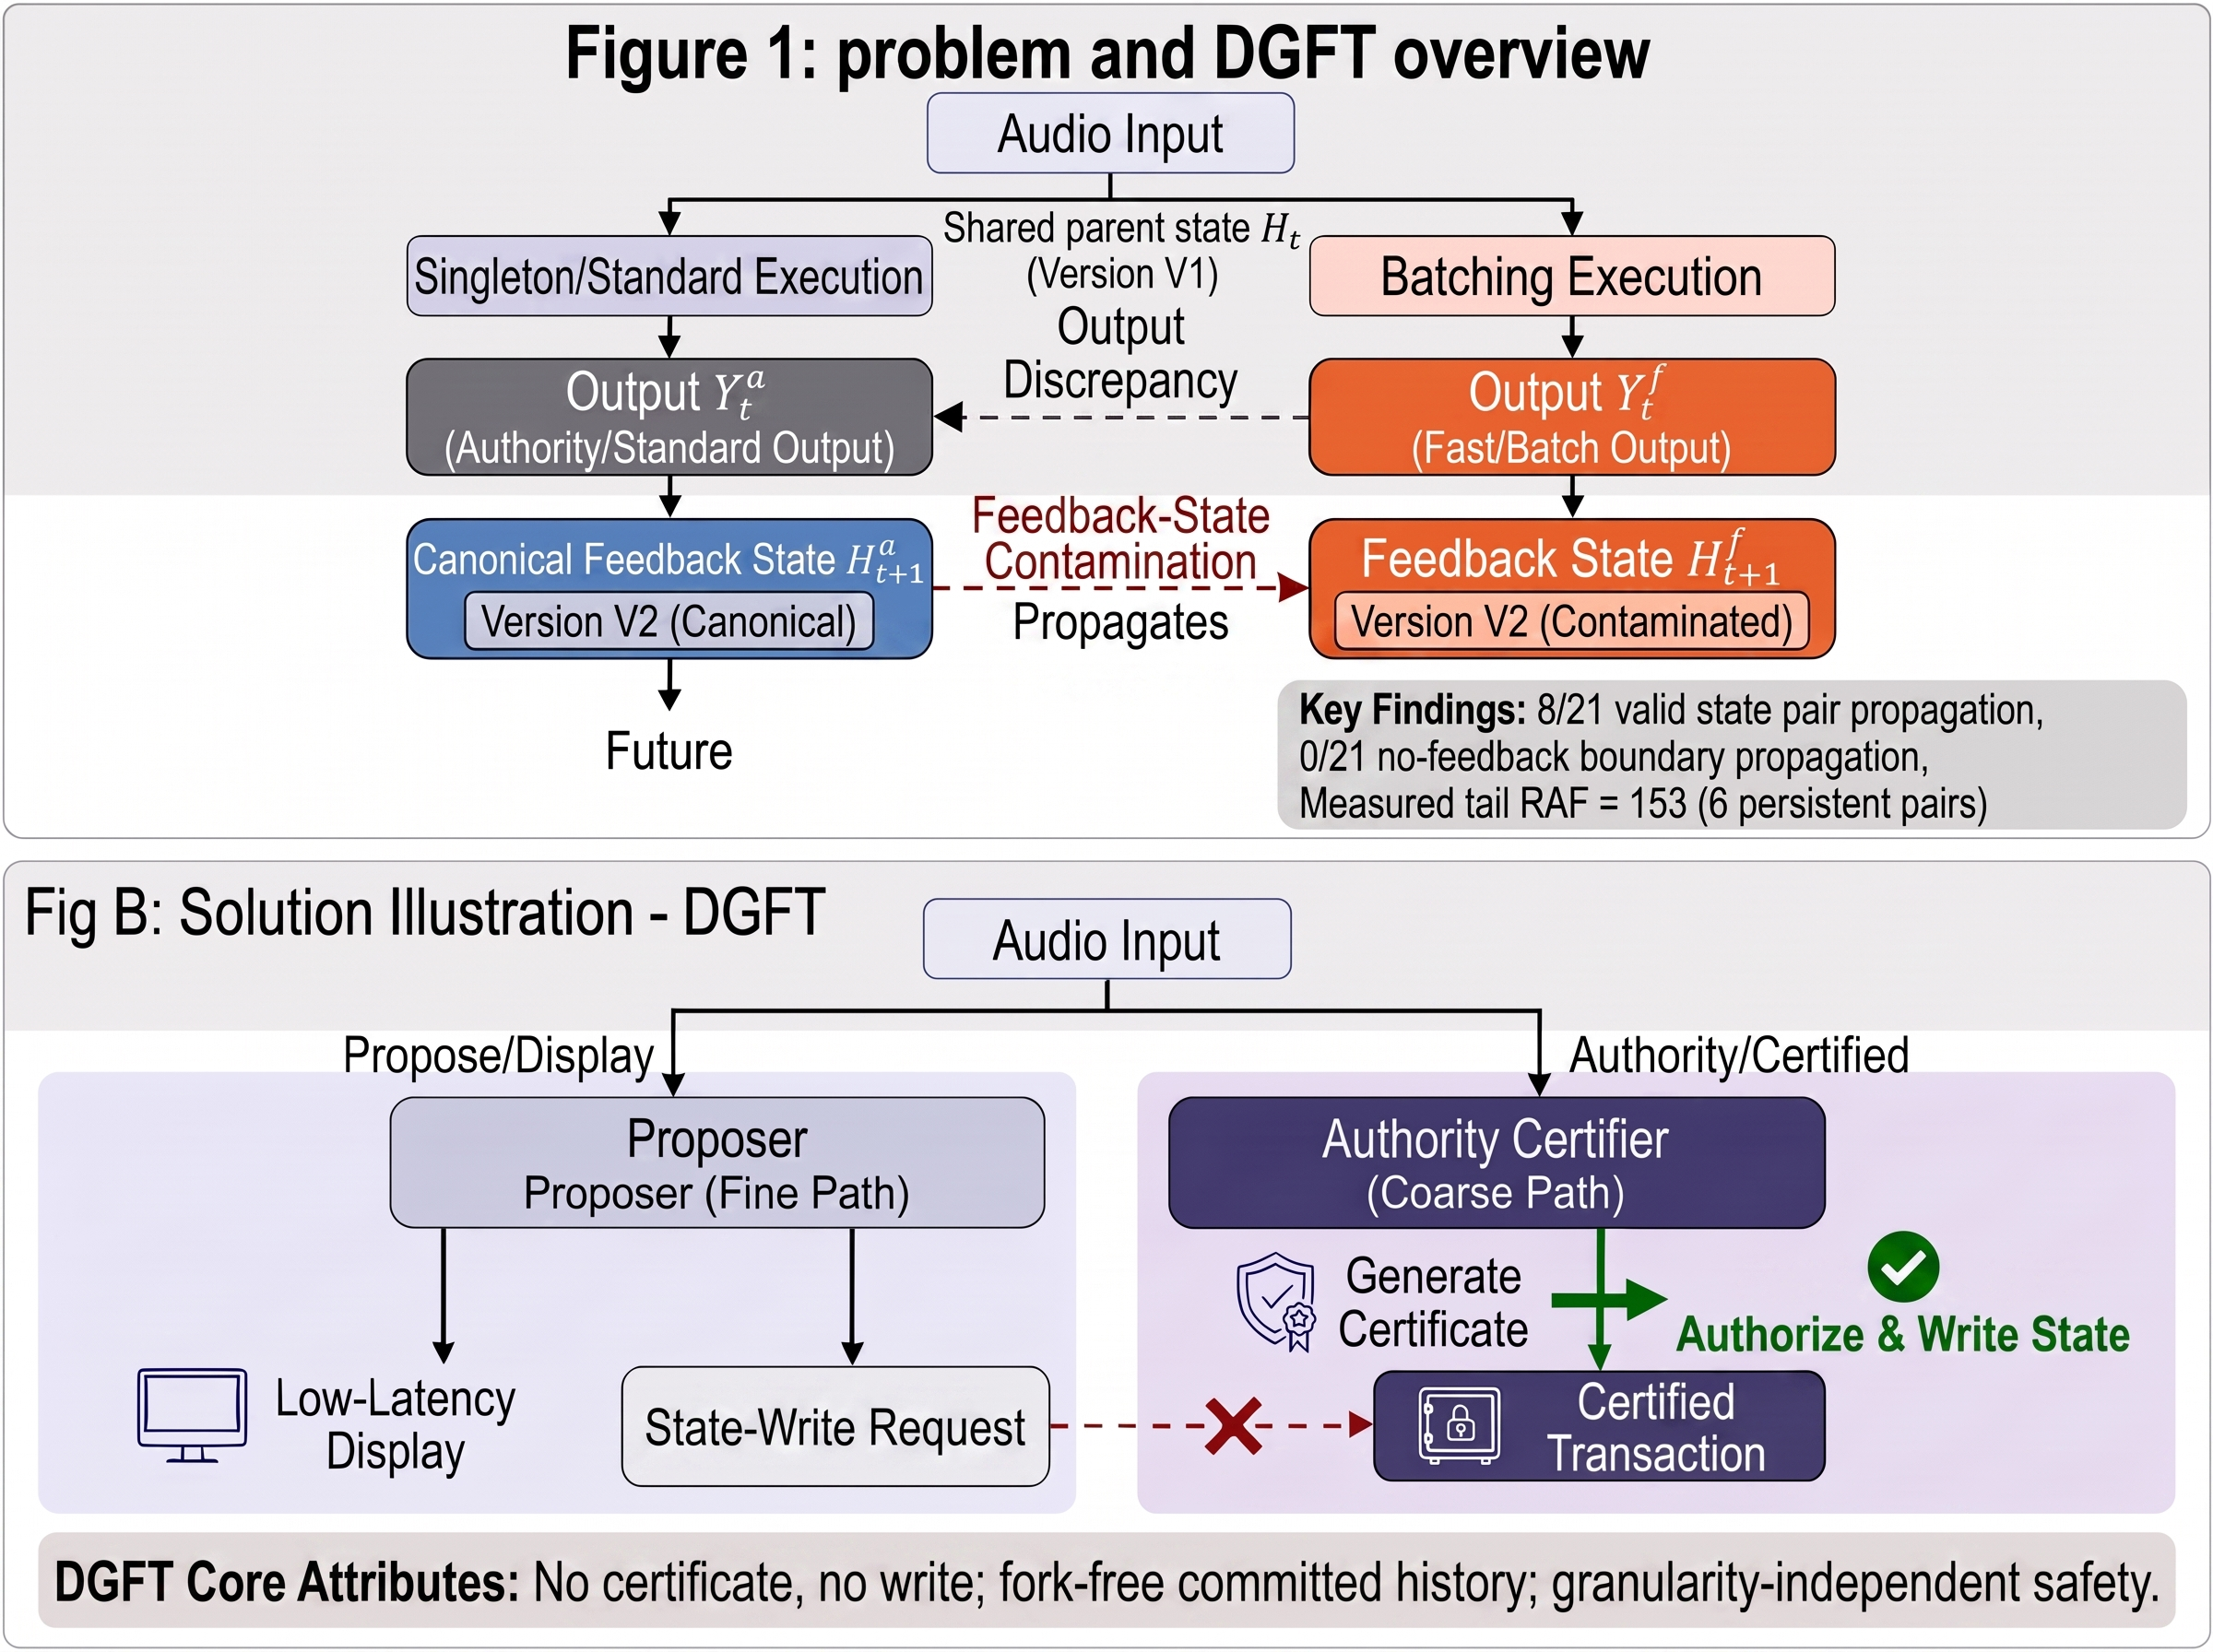
\includegraphics[width=0.96\textwidth]{figures/f1_motivation_senior.jpg}
  \caption{State-entry contamination under ordinary batching (a) and DGFT
  (b). Provisional outputs may differ; only certificate-authorized projections
  may become parents of future state.}
  \label{fig:motivation}
\end{figure*}

\subsection{Revision-generative state machines}\label{sec:model:rsm}

\begin{definition}[Revision-generative serving round]\label{def:rsm}
Round $t$ is $(\state_t,\audio_t,\out_t)$, where $\state_t$ is committed state,
$\audio_t$ is exogenous input (the audio frontier), and $\out_t$ is generated
output. Its update is
\begin{equation}\label{eq:state-update}
  \state_{t+1}=\mathcal{T}(\state_t,\audio_t,\out_t).
\end{equation}
The system is \emph{revision-generative} when $\mathcal{T}$ depends on
$\out_t$, so round $t$ affects state read by round $t{+}1$.
\end{definition}

\begin{definition}[Feedback sub-state and projection]\label{def:projection}
Write $\state_t=(\state_t^x,H_t)$, where $H_t$ is generated feedback and
$\state_t^x$ contains exogenous/runtime conditions held fixed in a causal
pair. The adapter projection $\proj$ writes
\begin{equation}\label{eq:feedback-update}
  H_{t+1}=\proj(\out_t;H_t),
\end{equation}
and the full update factors as
\begin{equation}\label{eq:state-update-h}
  \state_{t+1}=\mathcal{G}(\state_t^x,H_{t+1},\audio_t).
\end{equation}
For Qwen3-ASR, $H_t$ is the rollback prefix~\cite{shi2026qwen3asr}; for
Whisper with previous-text conditioning, it is the prompt~\cite{radford2023whisper}.
\end{definition}

The \emph{feedback edge} is the dependency
$\out_t\rightarrow H_{t+1}$ in Eq.~\eqref{eq:feedback-update}; removing it
makes the next feedback state independent of $\out_t$ while holding future
inputs and runtime assignments fixed. Ordinary batching instead installs
\begin{equation}\label{eq:implicit}
  H_{t+1}=\proj(\out_t^{\mathrm{batch}};H_t),
\end{equation}
without a separate state-write decision.

\subsection{Display output versus state projection}\label{sec:model:display}

Display-only suffixes, hold-back regions, and provisional hypotheses may be
visible while excluded from $\proj$ by the adapter. DGFT therefore enforces
the permission boundary
\begin{equation}\label{eq:invariant}
  \boxed{\mathrm{Display}(\out_t)\;\nRightarrow\;
  \mathrm{Authorize}(\proj(\out_t;H_t)).}
\end{equation}

\subsection{State-entry divergence and contamination}\label{sec:model:divergence}

For the same round, let $\out_t^f$ and $\out_t^a$ denote fine (batched)
proposal and canonical authority outputs.

\begin{definition}[Output divergence]\label{def:eps}
$\varepsilon_t=d_{\out}(\out_t^f,\out_t^a)$, where $d_{\out}$ is the
contract's output-space distance.
\end{definition}

\begin{definition}[State-entry divergence]\label{def:e}
For $P_t^f=\proj(\out_t^f;H_t)$ and
$P_t^a=\proj(\out_t^a;H_t)$,
$\ediv_t=d_{\state}(P_t^f,P_t^a)$ under the same mixed-unit metric.
\end{definition}

\begin{definition}[Contamination event]\label{def:contamination}
\[
  \cont_t \Longleftrightarrow \ediv_t>0\ \wedge\
  \proj(\out_t^f;H_t)\text{ is installed into }H_{t+1}.
\]
Thus output difference alone is not contamination; it must acquire
future-state write permission.
\end{definition}

\subsection{Feedback amplification}\label{sec:model:amplification}

Let $\dist_t=d_H(H_t^f,H_t^a)$ be trajectory distance under identical future
exogenous inputs and assignments.

\begin{assumption}[Local sensitivity]\label{ass:local}
Within the evaluated neighborhood of the canonical trajectory, finite
$L_t,\beta_t$ satisfy
\begin{equation}\label{eq:recurrence}
  \dist_{t+1}\le L_t\dist_t+\beta_t\ediv_t.
\end{equation}
The coefficients are unknown and the assumption makes no global Lipschitz
claim; the decomposition identifies propagation channels only.
\end{assumption}

\begin{remark}[Causal prediction]\label{rem:causal}
Removing the feedback edge sets $\beta_t=0$ for the intervened transition, so
an isolated state-entry perturbation cannot propagate through that edge when
future inputs, assignments, and arithmetic realizations are equal. A fresh
later divergence remains possible. Section~\ref{sec:eval} tests this scoped
prediction.
\end{remark}

\begin{definition}[Revision amplification factor]\label{def:raf}
For horizon $K$,
\[
  \mathrm{RAF}_{t,K}=\frac{\dist_{t+K}}{\ediv_t+\epsilon_0}
\]
is a measured trajectory indicator, not a theoretical bound.
\end{definition}

\subsection{Design requirements}\label{sec:model:reqs}

The model yields four requirements for certified feedback state:
\begin{description}
  \item[R1 (Authority separation).] Display and state-write permissions are
    distinct (Eq.~\eqref{eq:invariant}).
  \item[R2 (Parent ownership).] A projection commits only to the parent
    version against which it was computed.
  \item[R3 (Frontier monotonicity).] Committed audio intervals advance without
    gaps or overlap, forming one history.
  \item[R4 (Evidence non-authority).] Statistical evidence may schedule
    verification but never authorize installation.
\end{description}
Section~\ref{sec:dgft} realizes R1--R4 as protocol checks; Fig.~\ref{fig:arch}
and Table~\ref{tab:guarantees} trace them through the runtime and baselines.


\section{DGFT: Theory and Mechanism}\label{sec:dgft}
%% Section 3: DGFT --- theory and mechanism. Detailed protocol fields and
%% proofs appear in the accompanying Supplementary Material.

\subsection{Transactions, certificates, and commits}\label{sec:dgft:tx}

DGFT treats every projection written into the committed feedback sub-state
$H$ as a transaction; generated output never directly mutates $H$.

\paragraph{Trust model}
The authority coordinator and versioned ledger are trusted; proposers and
clients cannot mint or alter certificates. We assume collision-resistant
digests, immutable certified audio bytes, and atomic certificate consumption
with ledger compare-and-swap. A digest binds content but does not authenticate
it independently; authenticity follows from protected authority issuance. We
exclude Byzantine authorities and compromised ledgers. The protocol requires
neither deterministic proposers nor synchronous GPU execution: the authority
may use any decoding policy whose realized projection and complete runtime
configuration, including its randomness policy, are bound by the certificate.
Asynchronous completions remain safe because the parent-version
compare-and-swap serializes installation. These assumptions certify provenance
and write legality, not semantic correctness or repeatability of an
independently rerun stochastic authority.

\begin{definition}[DGFT transaction]\label{def:tx}
A transaction is
\[
  \tx_t=(\mathrm{sid},e,p,v_{\mathrm{parent}},[a_s,a_e),\out_t,
  \proj(\out_t;H_t),\mathrm{cert}_t),
\]
where the fields identify the session, contract epoch, policy, parent version,
covered audio frontier, output, state projection, and certificate. Proposal
and authority granularities $g_p$ and $g_a$ define
$\granratio=g_a/g_p\geq1$.
\end{definition}

\begin{definition}[Certificate]\label{def:cert}
For canonical projection $\proj_j^a=\proj(\out_j^a;H_{v_j})$, the authority
issues the single-use record
\[
\begin{aligned}
 \cert_j=\mathrm{Bind}\bigl(&\mathrm{sid}_j,e_j,p_j,v_j,\\[-2pt]
 & [f_j,f_{j+1}),h(\audio_{[f_j,f_{j+1})}),\\[-2pt]
 & h(\proj_j^a),\chi_j\bigr),
\end{aligned}
\]
where $\chi_j$ binds the checkpoint, tokenizer, decoding policy, projection
adapter, precision, and authority-runtime version. Thus one certificate names
exactly one canonical projection and commit context.
\end{definition}

\begin{definition}[Commit validity]\label{def:commit}
For
\[
\begin{aligned}
 \commit_j=(\mathrm{sid}_j,e_j,p_j,v_j,&[f_j,f_{j+1}),\\[-2pt]
 &\proj_j^a,\cert_j),
\end{aligned}
\]
the commit is valid iff: (i) its session, epoch, and policy match the
live fence; (ii) $v_j$ is the committed parent; (iii) its frontier is the next
gap- and overlap-free interval; and (iv) the unconsumed certificate binds all
presented fields and the recomputed projection digest. Only valid commits
mutate $H$.
\end{definition}

These checks realize R1--R4 (Section~\ref{sec:model:reqs}): display creates no
commit, parent and frontier are checked at installation, and risk evidence
never issues a certificate. Table~\ref{tab:guarantees} contrasts this contract
with weaker regimes. Binding $\chi_j$ is essential: a result from another
checkpoint, tokenizer, precision, or decoder policy cannot be replayed as if it
were produced by the live canonical contract.

\tbl{t5_guarantees}

\begin{definition}[Committed provenance ancestry]\label{def:ancestry}
A projection is an ancestor of $H_j$ iff it labels an accepted transition on
the unique ledger path $H_0\rightarrow\cdots\rightarrow H_j$; displayed or
rejected projections are not ancestors.
\end{definition}

\subsection{Theorem 1: uncertified-ancestry exclusion}\label{sec:dgft:thm1}

\begin{theorem}[Uncertified-Ancestry Exclusion]\label{thm:ancestry}
If $H$ changes only through valid commits, no fine projection unbound by a
valid certificate can enter the ancestry of any future committed state.
\end{theorem}

\begin{proof}[Proof sketch]
Induct over accepted commits. $H_0$ has no generated ancestor. A valid next
commit installs exactly the projection digest bound by its certificate;
different content fails validation, while display does not mutate $H$.
Therefore the invariant is preserved. The full proof, including the case in
which proposal and authority projections coincide, is in Supplementary
Section~S2.
\end{proof}

The result depends on commit provenance, not margins, model determinism,
precision agreement, or ASR architecture.

\subsection{Theorem 2: fork-free committed-state linearity}\label{sec:dgft:thm2}

\begin{theorem}[Fork-Free Committed-State Linearity]\label{thm:linear}
If validation and installation form one atomic compare-and-swap and each
certificate is consumed at most once, parent-version and frontier checks make
the accepted commits of a session a fork-free, gap-free, overlap-free linear
history.
\end{theorem}

\begin{proof}[Proof sketch]
Atomic compare-and-swap prevents two commits from installing against the same
parent. Parent checking rejects stale branches, single-use certificates reject
replay, and frontier continuity orders the remaining intervals without gaps
or overlaps. See Supplementary Section~S2 for the stepwise argument.
\end{proof}

\begin{remark}[Scope of the concurrency claim]\label{rem:not-linearizable}
The ledger compare-and-swap serializes accepted commits. This is not full
Herlihy--Wing linearizability of all client operations, which would require a
real-time concurrent-object specification~\cite{herlihy1990linearizability}.
\end{remark}

\begin{corollary}[Stale-descendant rejection]\label{cor:stale}
Any revision with $v_{\mathrm{parent}}\neq\mathrm{version}(H_j)$ fails the
parent check and cannot mutate state.
\end{corollary}

\subsection{Theorem 3: granularity-independent safety}\label{sec:dgft:thm3}

\begin{theorem}[Granularity-Independent Safety]\label{thm:gran}
For any $\granratio\geq1$, if each authority segment begins at the committed
parent, covers the next contiguous frontier, produces a legal projection, and
passes certificate and version checks, Theorems~\ref{thm:ancestry}
and~\ref{thm:linear} hold.
\end{theorem}

\begin{proof}[Proof sketch]
Both proofs depend only on binding, validity, and atomic installation; changing
$\granratio$ changes certificate coverage, not admissibility.
\end{proof}

\begin{corollary}[Same-granularity certification as $\granratio=1$]\label{cor:sg}
At $\granratio=1$, proposal and authority regions coincide: directional
coverage becomes identity and fine replay becomes risk-triggered
re-verification. SG is therefore a protocol reduction of DGFT.
\end{corollary}

\begin{remark}[Canonical-path boundary]\label{rem:canonical}
This reduction is protocol-level. Our SG contract uses FP16 singleton
authority, whereas Coarse/Hybrid use FP32 batched authority; we never claim
bitwise identity between these canonical paths.
\end{remark}

\subsection{Authority-cost decomposition}\label{sec:dgft:cost}

Let $B$ denote concurrent sessions, $q$ the SG verification fraction, $r$ the
Hybrid replay fraction, $C_s$ singleton authority cost per fine region,
$C_c(\granratio,B)$ batched coarse cost, $C_{\mathrm{commit}}$ transaction
overhead, and $Q_s$ singleton queueing/fragmentation cost. Then
\begin{align}
 T_{\mathrm{SG}}^a&\approx qB\granratio C_s+Q_s,\label{eq:cost-sg}\\
 T_{\mathrm{DGFT}}^a&\approx C_c(\granratio,B)+rB\granratio C_s+
 C_{\mathrm{commit}},\label{eq:cost-dgft}
\end{align}
and, with separate proposer and authority GPUs,
\begin{equation}\label{eq:cost-service}
 T_{\mathrm{service}}\approx\max(T_p,T^a)+T_{\mathrm{repair}}.
\end{equation}

\begin{proposition}[Model-based operating condition]\label{prop:coarse}
When authority is on the critical path and repair costs are comparable,
Coarse-DGFT improves throughput over SG if
\[
 C_c(\granratio,B)+rB\granratio C_s+C_{\mathrm{commit}}
 <qB\granratio C_s+Q_s.
\]
\end{proposition}

The model predicts that even small $q$ can create singleton tails, whereas a
coarse authority may amortize invocation and queueing. Hybrid trades replay
for quality, and model-dependent authority paths can reverse the ordering.
Section~\ref{sec:eval:rq3} tests these predictions; because the evaluated
canonical paths differ (Remark~\ref{rem:canonical}), results identify complete
operating points rather than a precision-independent effect of $\granratio$.
The decomposition is therefore an explicit performance model, not part of the
safety proof and not an assertion that coarse authority is always faster.

\subsection{Operating-point trade-offs}\label{sec:dgft:tradeoff}

Deployment selects SG, Coarse, or Hybrid to maximize an objective $J(\pi)$
subject to zero transaction violations and contract caps:
\[
 \max_{\pi}J(\pi)\quad\text{s.t.}\quad V(\pi)=0,\;C(\pi)\leq B.
\]
DGFT defines this safe envelope; it does not claim that one measured operating
point dominates across workloads or models.


\section{The RevTrace Runtime}\label{sec:system}
%% Section 4: RevTrace system.

RevTrace realizes DGFT with family adapters, a two-plane coordinator, a
versioned ledger, and contract-scoped certification (Fig.~\ref{fig:arch}).

\begin{figure*}[t]
  \centering
  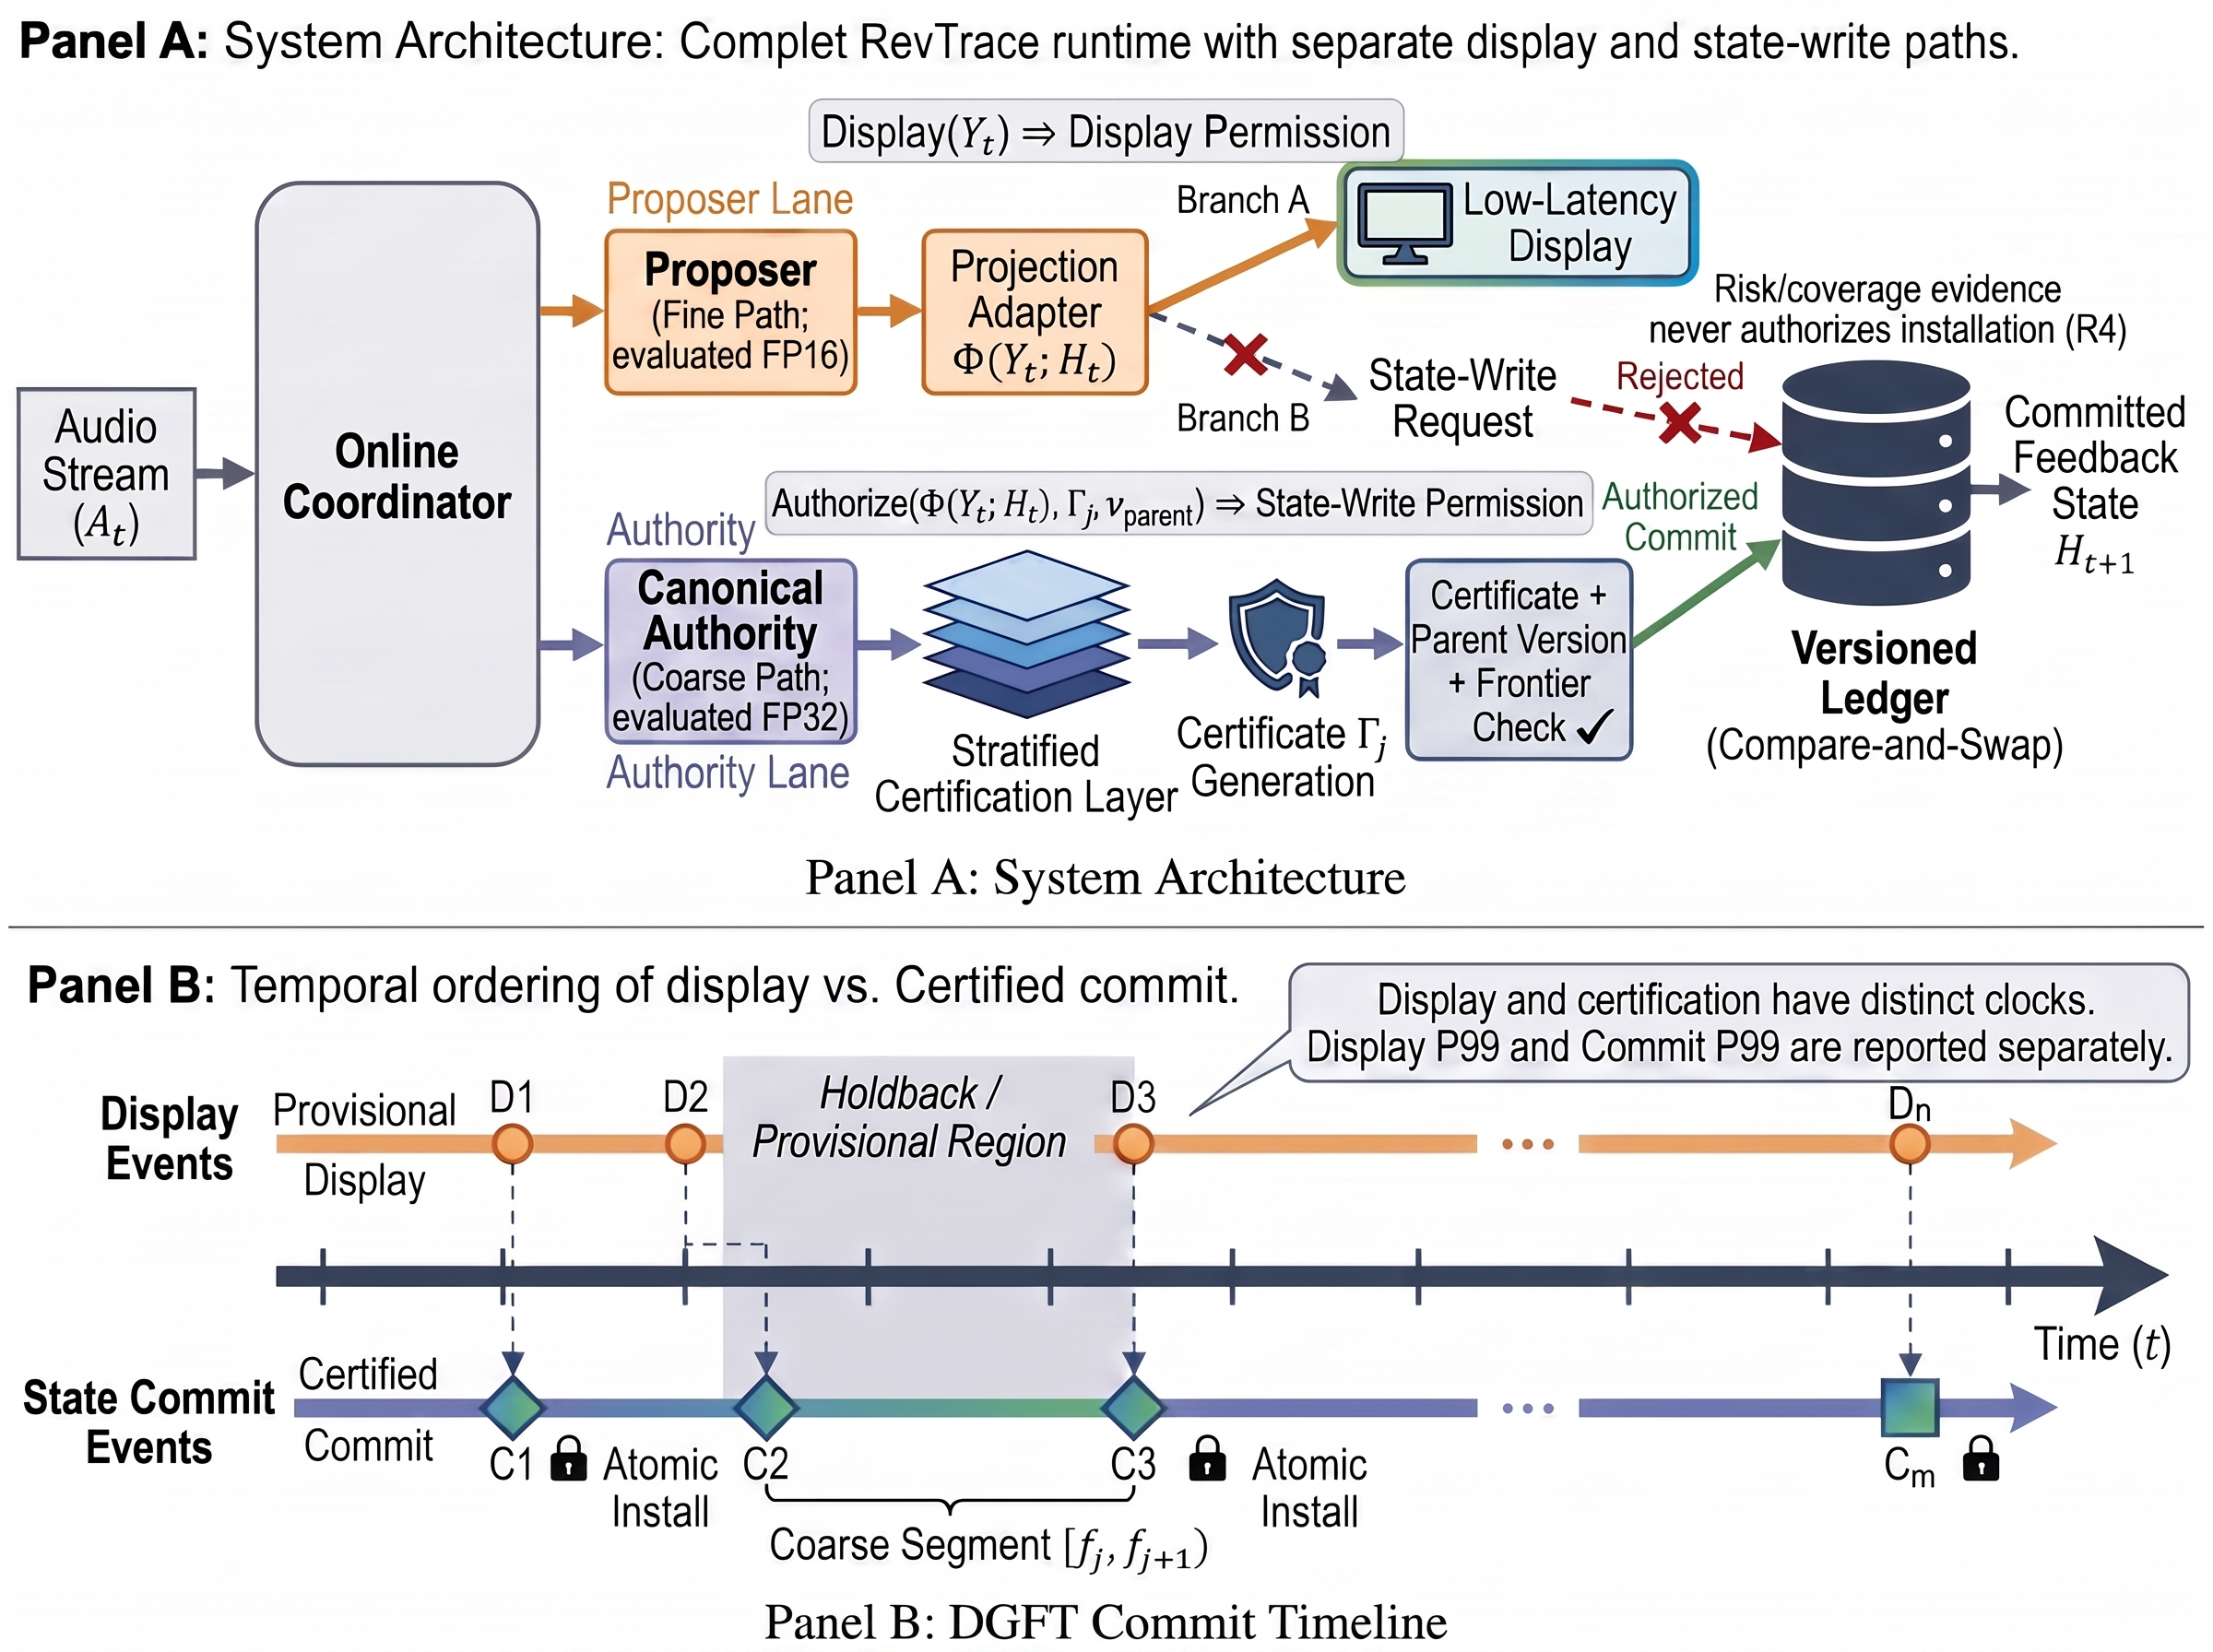
\includegraphics[width=0.94\textwidth]{figures/f2_architecture_senior.jpg}
  \caption{RevTrace architecture and commit timeline. Proposal may drive
  low-latency display, but only a certificate bound to the current parent and
  frontier may install state. FP32 is the evaluated coarse authority, not a
  protocol requirement.}
  \label{fig:arch}
\end{figure*}

\subsection{Adapters and two-plane coordination}\label{sec:sys:adapters}

Each model family supplies three interfaces: a projection adapter computing
$\proj(\out_t;H_t)$ (Qwen rollback prefix or Whisper previous-text prompt), an
authority adapter executing its canonical path, and an evidence adapter that
collects margins, directional coverage, and repetition signals. The online
coordinator runs proposer and authority on separate GPUs, invalidates stale
descendants (Corollary~\ref{cor:stale}), closes terminal frontiers, and rebases
displayed provisional state after superseding commits. RQ3 evaluates the same
runtime through both family adapters. A slow authority may delay certified
commit without blocking provisional display; the evaluation consequently
reports display and commit clocks separately.\label{sec:sys:coord}

\subsection{Certificate ledger}\label{sec:sys:ledger}

The compare-and-swap ledger stores the committed version and audio frontier.
Before installation it matches each $\commit_j$ against the session, contract
epoch, policy, parent-version, frontier, and certificate-consumption fences.
RQ2 exhaustively records these checks for every install attempt.

\subsection{Coverage and selective replay}\label{sec:sys:coverage}

A coarse certificate records, in Latin or CJK units, which proposal regions it
covers. Uncovered regions enter fine replay; Hybrid additionally replays
risk-selected regions at fraction $r$. Coverage therefore controls work but
does not grant write authority. RQ3 compares Coarse ($r=0$) and Hybrid ($r>0$)
under a matched workload.

\subsection{Stratified certification}\label{sec:sys:cert}

The four non-transferable strata in Fig.~\ref{fig:cert} are: (i) randomized,
anytime-valid UCB audits of SG numerical risk, scoped only to the SG adapter
path~\cite{howard2021confidence,ramdas2023savi}; (ii) fail-closed,
contract-scoped preflight tests of authority repeatability and
batch-vs-singleton invariance; (iii) exhaustive online certificate, version,
and frontier validation; and (iv) independent family-specific semantic
references. Evidence may schedule verification but never authorize a state
write (R4). The separation prevents a favorable statistical bound in one
contract from being promoted into an installation certificate for another.

\begin{figure*}[t]
  \centering
  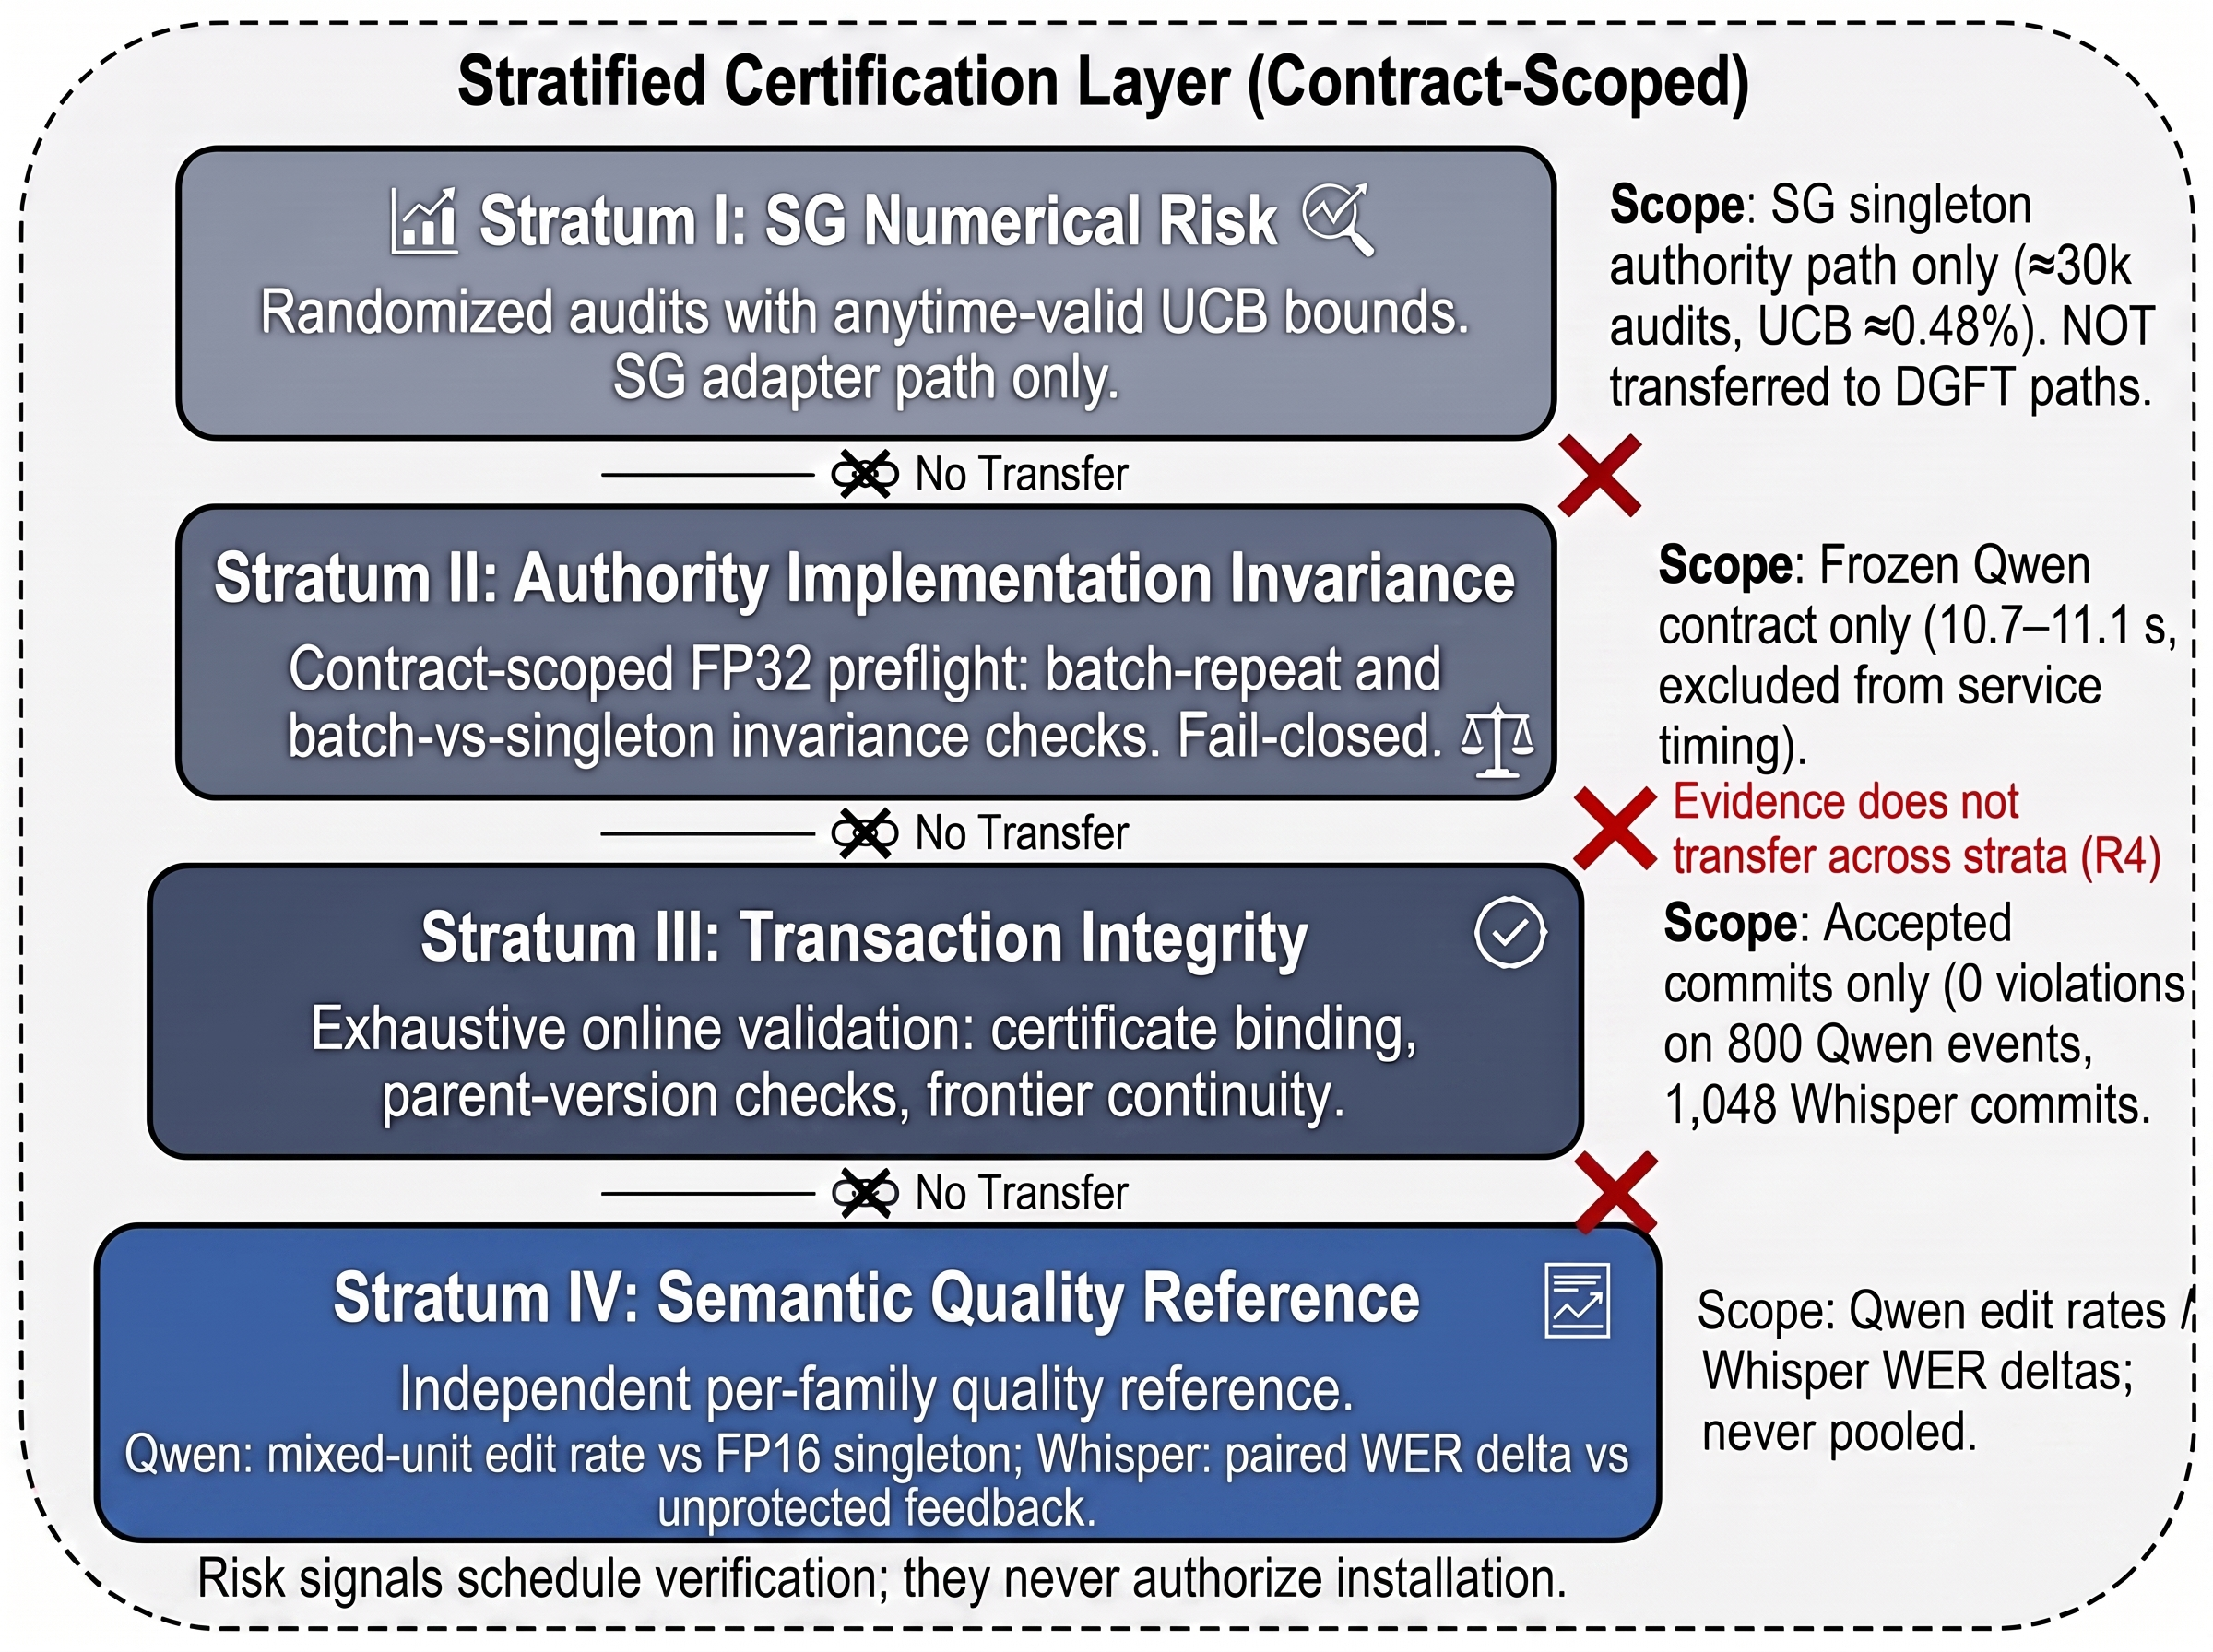
\includegraphics[width=0.92\textwidth]{figures/f3_certification_senior.jpg}
  \caption{Contract-scoped certification. Each stratum supports only its stated
  guarantee; evidence never transfers across strata. Qwen and Whisper quality
  estimands remain separate.}
  \label{fig:cert}
\end{figure*}


\section{Implementation}\label{sec:impl}
%% Section 5: Implementation.

RevTrace supports Qwen rollback-prefix and Whisper previous-text adapters with
growing audio and holdback semantics~\cite{shi2026qwen3asr,radford2023whisper}.
In the frozen implementation, SG uses FP16 singleton authority and
Coarse/Hybrid use FP32 batched authority with a 4{,}096-token per-session
KV-cache bound. The latter's 10.7--11.1\,s one-time fail-closed preflight is
reported separately and excluded from steady-state timing. FP32 is not a DGFT
requirement: replacing it requires a new canonical contract and the same
preflight and quality checks.

The primary deployment uses two RTX~3090 GPUs, one per plane, causal arrivals,
and vectorized host transfer. The independent scale contract uses one
RHEL~7.6 node with eight 32-GB V100 PCIe GPUs, PyTorch~2.4.1, CUDA~12.1, and
Transformers eager execution. It runs up to four proposer and four authority
replicas over a shared versioned commit queue---not distributed model
parallelism. Audio is deterministically resampled to 16\,kHz. Contract
fingerprints, rejected realizations, raw records, and result hashes remain in
the release; timing is never pooled across hardware contracts. Each reported
run is bound to a code revision and contract digest so that protocol changes
cannot be mixed with frozen measurements.
\artifactavailability


\section{Evaluation}\label{sec:eval}
%% TC adaptation: seven internal hypotheses are consolidated into four RQs.
%% Numeric evidence remains bound to its frozen hardware/workload/quality contract.

\subsection{Setup and Research Questions}\label{sec:eval:setup}

We evaluate five checkpoints from two revision-generative ASR families:
Qwen3-ASR 0.6B/1.7B and Whisper tiny/base/small.en. The main system runs use
two RTX~3090 GPUs. The matched comparison uses the same 16 bilingual 30-s
sessions (c16; 480\,s of audio), whereas cross-family production results retain
their original family-specific workloads and references. Scale-out is measured
separately on one RHEL~7.6 node with eight 32-GB Tesla V100 PCIe GPUs and the
Transformers-eager backend. Quality is evaluated against an independent
canonical replay for Qwen and unprotected feedback for Whisper. We never pool
results across hardware, families, authority paths, or quality estimands.

\emph{Metrics and timing.} Audio xRT is completed audio seconds divided by
service wall time. Wall speedup divides singleton-reference wall time by
service wall time; GPU-normalized speedup additionally divides by the
service-to-reference GPU-count ratio (two for the RTX~3090 cells). Energy is
trapezoidally integrated from NVIDIA Management Library (NVML) power samples
and normalized by completed
audio seconds. Display latency measures ready-to-proposal completion, whereas
state/segment-commit latency measures ready-to-authorized installation; the two
clocks are never interchanged. Timed cells use immutable causal arrival
schedules, while wall and energy meters record real execution. The matched
Qwen cells use 2-s fine revisions and 6-s authority segments
($\granratio=3$). ``16/16 pass'' means that every Whisper production cell met
its frozen thresholds: wall speedup $\ge2.5\times$, GPU-normalized speedup
$\ge1.25\times$, energy reduction $\ge20\%$, display P99 $\le1.9$,s, commit
P99 $\le36$,s, audio amplification $\le1.2\times$, and zero semantic
violations.

The evaluation asks: \emph{RQ1}, does the feedback edge causally propagate a
local execution difference? \emph{RQ2}, does DGFT preserve transaction
integrity? \emph{RQ3}, what performance--quality--energy frontier does the
authority split expose, including against the nearest adapted baselines?
\emph{RQ4}, how does independent proposer/authority replication scale?

\subsection{RQ1: Causal Propagation}\label{sec:eval:rq1}

We enumerate 21 legal Whisper state pairs and apply the same isolated
batch-created divergence with the feedback edge present and removed, while
holding future inputs, batch assignments, and arithmetic realization fixed.
With feedback, 8/21 pairs propagate; without feedback, 0/21 do. Six pairs
remain divergent into the measured tail, where the revision amplification
factor (Definition~\ref{def:raf}) reaches 153. This intervention identifies
feedback as the propagation channel; it does not estimate a production
prevalence.

\subsection{RQ2: Transaction Integrity}\label{sec:eval:rq2}

We validate every accepted install in 800 Qwen events (480 SG and 320 DGFT)
and 1{,}048 Whisper commits. Under the trust and binding assumptions of
Section~\ref{sec:dgft}, all completed sessions have monotone terminal frontiers,
with zero observed transaction-install, output/state, stale-result, or replay
violations. No stale install was attempted in these production traces; hence
they validate accepted-history integrity rather than fault-injected stale
rejection.

A deterministic state-machine fuzzer supplies the adversarial complement. It
issues 250{,}000 attempts across 64 sessions and 24 invalid/replay classes,
including cross-session and cross-epoch substitution, certificate tampering,
stale parents, frontier gaps/overlaps, duplicates, and replays. The runtime
accepts all 10{,}000 valid commits and rejects all 240{,}000 mutations, with no
invariant violation. This is exhaustive validation over the evaluated traces
and mutation suite, not a zero-failure-probability claim; it excludes Byzantine
trusted components, GPU worker crashes, and wall-clock expiry.

To isolate transaction logic from accelerator execution, we benchmark the
production commit primitive on the submission host using 31 randomized
repeats of 20{,}000 valid calls (2{,}000-call warmup; 256-token prompt,
32-token display, and eight speculative descendants). The median full commit
is 101.107\,$\mu$s versus 19.077\,$\mu$s for the same immutable-state
materialization without checks, a paired incremental cost of
81.960\,$\mu$s/commit; the full-commit P99 across repeat aggregates is
104.514\,$\mu$s. This host-side protocol microbenchmark is not GPU or
end-to-end speedup evidence; Supplementary Section~S4 gives all variants and
the existing online critical-section cross-check.

\subsection{RQ3: Service Frontier, Quality, and Baselines}
\label{sec:eval:rq3}

\paragraph{Matched authority configurations}
Figure~\ref{fig:ablation} compares complete configurations on the identical c16
workload: SG ($\granratio=1$, FP16 singleton authority), Coarse-DGFT
($\granratio=3$, FP32 batched authority), and Hybrid-DGFT
($\granratio=3$ plus selective replay). Authority precision, execution mode,
and granularity change together, so this is not a precision-independent
ablation of $\granratio$.

\begin{figure}[t]
  \centering
  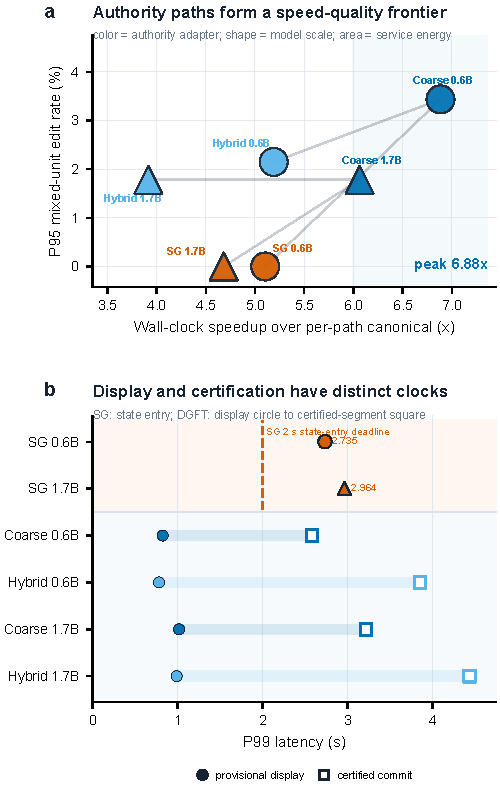
\includegraphics[width=\columnwidth]{figures/f3_authority_frontier_column.pdf}
  \caption{Matched c16 authority configurations. Marker area denotes energy;
  display and certified-commit latencies remain distinct estimands.}
  \label{fig:ablation}
\end{figure}

Coarse reduces service wall time from 14.905 to 10.759\,s (0.6B) and from
16.285 to 12.763\,s (1.7B), giving direct throughput gains of
$1.39\times$ and $1.28\times$ over SG. Its separately normalized headline
speedups are $6.88\times/6.06\times$ over each path's frozen all-singleton
reference; these normalizations are not divided to obtain the matched ratios.
SG's synchronized terminal burst yields certified state-entry P99
2.735/2.964\,s and 2-s miss rates 3.33\%/4.17\%. Coarse/Hybrid instead expose
display P99 $\le1.018$\,s and segment-commit P99 2.582--4.437\,s. Coarse energy
relative to SG changes from $-4.4\%$ on 0.6B to $+15.1\%$ on 1.7B; Hybrid costs
$+16.8\%/+54.2\%$. The reversal confirms that the complete authority path,
not granularity alone, determines the operating point.

\paragraph{Cross-family production and quality}
On Qwen, Coarse-DGFT reaches $6.88\times/6.06\times$ wall speedup,
$3.44\times/3.03\times$ GPU-normalized speedup, and 59.8\%/51.0\% energy
reduction for 0.6B/1.7B. On Whisper, the same transaction runtime passes all
16 production cells: median wall speedup is $2.841\times$ (range
2.633--3.849), GPU-normalized speedup is $1.421\times$, median energy reduction
is 31.13\%, and display P99 is at most 1.492\,s. Figure~\ref{fig:production}
reports each family against its own baseline; the magnitudes are not compared
across columns.

\begin{figure*}[t]
  \centering
  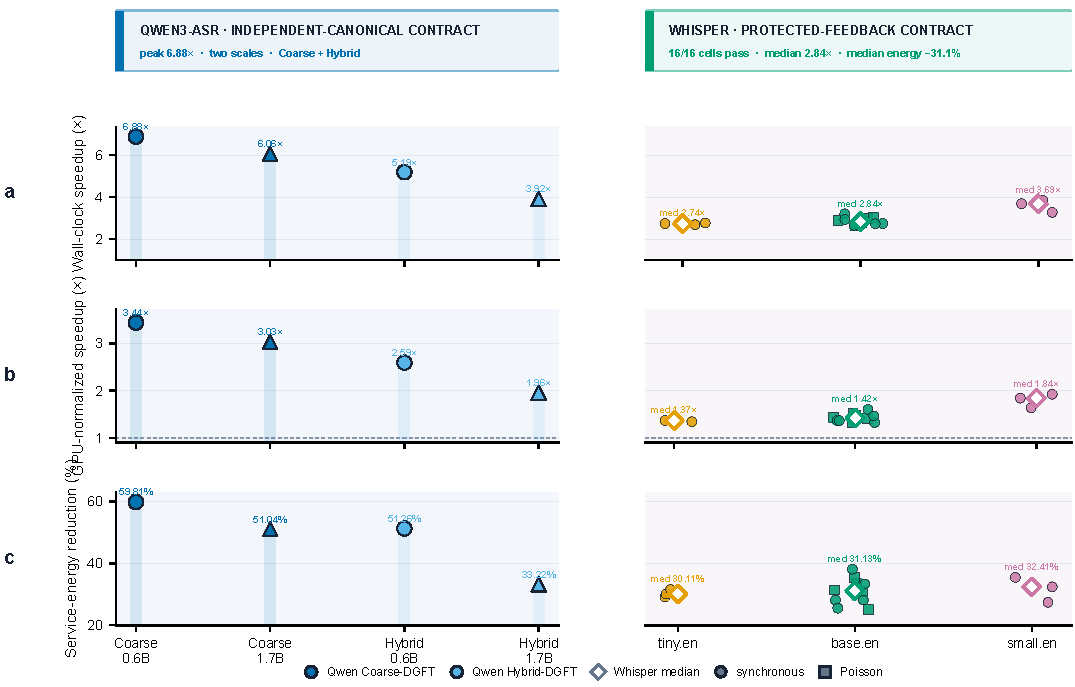
\includegraphics[width=\textwidth]{figures/f4_production.pdf}
  \caption{Production performance under family-specific contracts. Qwen and
  Whisper use different baselines and are not pooled.}
  \label{fig:production}
\end{figure*}

Qwen's mixed-unit edit rate against independent FP16 singleton replay has
empirical P95 $\le3.43\%$ (worst session 5.41\%; no catastrophic case). On
deterministic 64-utterance holdouts from \emph{LibriSpeech test-clean} and
\emph{AISHELL-1}, respectively, 0.6B/1.7B obtain English WER
2.15\%/2.30\% and Chinese CER 2.71\%/2.16\%, with 256/256 terminal outputs
exactly matching singleton authority and partial-revision edit rates
24.7--31.8\%. These are fixed holdouts, not full-corpus leaderboard results.

For Whisper, protection improves WER relative to unprotected feedback for
tiny/base/small.en by $-12.23/-18.21/-25.27$ points on development sessions
and $-8.26/-11.03/-13.76$ on the untouched cohort. All one-sided 95\%
bootstrap upper bounds remain below zero. The untouched cohort contains 40
long sessions per model, deterministically assembled from 214 previously
unused source utterances; the long session is the bootstrap unit. These
family-specific quality questions remain separate (Figure~\ref{fig:quality}).

\begin{figure}[t]
  \centering
  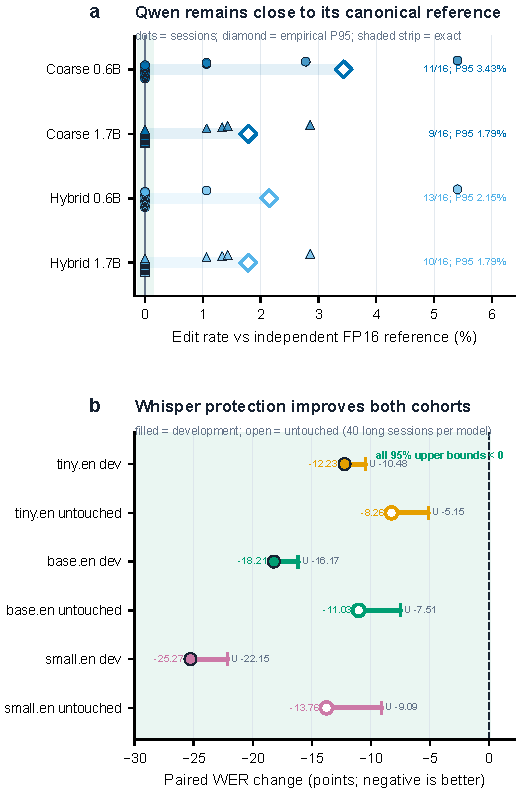
\includegraphics[width=\columnwidth]{figures/f5_quality_column.pdf}
  \caption{Family-specific quality. Qwen measures edit distance to an
  independent canonical replay; Whisper measures paired WER change from
  unprotected feedback.}
  \label{fig:quality}
\end{figure}

\paragraph{Nearest adapted baselines}
Table~\ref{tab:normal-adaptations} compares all methods on the independent
V100 c16 workload; all 240 display events per cell meet the 2-s display SLO.
Against an LLM-42-style revision adaptation that verifies every revision,
Coarse-DGFT improves audio throughput by $6.91\times/5.64\times$ on
0.6B/1.7B. Against MarginGate-inspired scheduling, Coarse is 5.6\% slower on
0.6B and 11.5\% faster on 1.7B. The latter has no state-write authorization
contract, so this comparison quantifies normal-load cost rather than equivalent
safety.

\tbl{t8_normal_slo_adaptations}

On a separate overloaded c32 stress trace, MarginGate-inspired verification
checks 3.02\% of events but misses the known state-changing flip; an
owner/version-only fence also accepts it. Always-verifying LLM-42-style replay
removes the error at 1.565 events/s, whereas RevTrace verifies 5.05\%, removes
the error, and reaches 3.046 events/s ($1.95\times$). Because P99 is
6.107\,s, this trace measures safety cost, not serving capacity. A legal
execution-shape suite (batch size, slot, composition, and repeat) induces
1{,}021 proposal--canonical mismatches among 1{,}848 target-row evaluations;
the frozen risk scheduler has zero observed false-safe events. Risk schedules
verification but never certifies a write~\cite{chu2026margingate,zhang2026llm42}.

\subsection{RQ4: Replica Scaling and Capacity}\label{sec:eval:rq4}

The independent V100 study contains 84 cells spanning authority
microprofiles, c16 baselines, c16--c128 replica allocations, and
$\granratio\in\{1,3,5\}$ attribution. We freeze the headline allocations and
repeat 30 additional cells (three runs per model and configuration); ranges in
Figure~\ref{fig:v100-dual-plane} are min--max. Repeated batched executions
agree, but each model still has 62 batch--singleton request mismatches across
precisions and batch sizes. FP32 batching is therefore a contract-scoped
authority, not an unconditional singleton-equivalence certificate.

At c16, SG/Hybrid/Coarse reach $4.682/5.764/6.072\times$ wall speedup on
0.6B and $3.248/4.657/4.893\times$ on 1.7B. Balanced four-proposer plus
four-authority replication at c64 sustains median $157.786\times/111.722\times$
audio real-time throughput. Display P99 is 1.089/1.394\,s with zero misses
over 2{,}880 repeated events per model; certified-segment commit P99 is
separately 3.080/4.890\,s. At c128, display P99 rises to 2.079/2.730\,s and
commit P99 to 6.012/10.153\,s, while throughput saturates. Thus c64 is the
largest measured point satisfying the display SLO for both models, and c128 is
retained as the failed boundary.

An authority-heavy 3+5 allocation at c64 lowers the authority/proposer service
ratio but also lowers throughput to $93.788\times/77.704\times$ and yields
display P99 1.756/2.209\,s; adding authority replicas does not repair the
proposer bottleneck, and balanced 4+4 dominates. At
$\granratio=1$, FP32 authority/proposer ratios 2.216/2.669 reduce throughput to
$18.603\times/12.294\times$; at $\granratio=5$, the ratios fall below one and
throughput recovers to $40.630\times/33.909\times$. These results support the
two-stage cost model: balanced replication expands capacity, while coarse
authority becomes economical only after sufficient amortization. They
establish single-node, not multi-node, scaling.

\begin{figure*}[t]
  \centering
  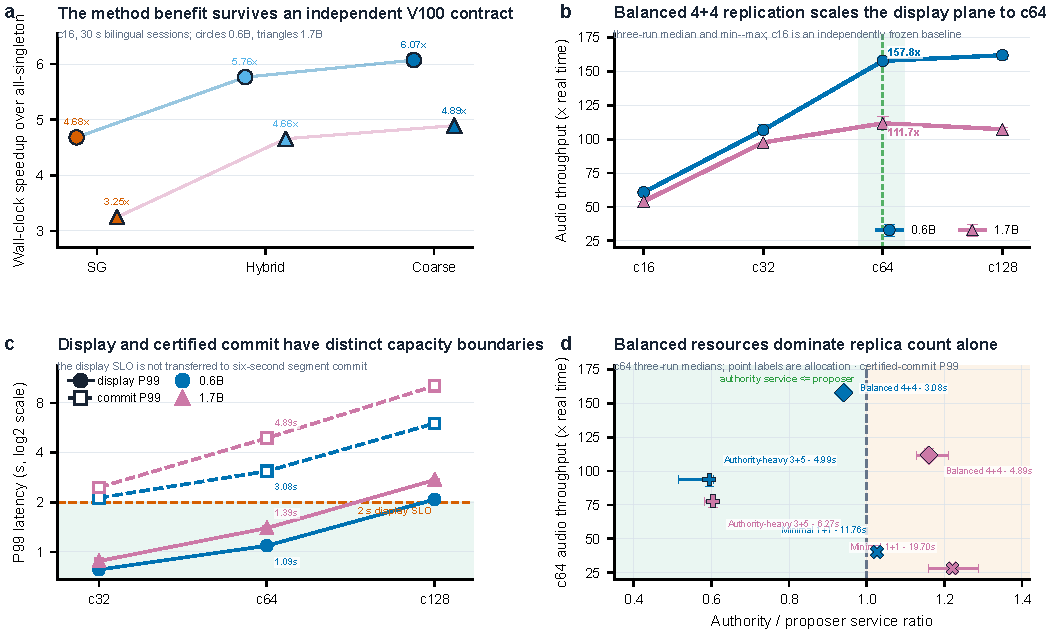
\includegraphics[width=\textwidth]{figures/f7_v100_dual_plane.pdf}
  \caption{Independent V100 replica scaling. Balanced 4+4 reaches the c64
  display-SLO boundary; display and certified-commit latency are reported on
  distinct clocks. Points at c32--c128 show three-run medians and min--max
  ranges.}
  \label{fig:v100-dual-plane}
\end{figure*}


\section{Discussion and Boundaries}\label{sec:discussion}
%% TC adaptation: compact interpretation and explicit scope boundaries.

\paragraph{Authority semantics and evidence boundaries}
FP32 batching is the canonical authority for the declared Coarse/Hybrid
contract, not a bitwise repair of the FP16 proposer. DGFT requires an authority
that emits a contract-bound projection and certificate; it does not require a
particular precision. A deterministic low-precision kernel portfolio or
canonical replay could replace FP32 only after a new contract epoch passes its
own validation. The 10.7--11.1\,s Qwen preflight is therefore reported once and
excluded from service timing. Likewise, the SG adapter's 0.480\% anytime-valid
UCB over approximately 30{,}000 randomized audits does not transfer to
Coarse/Hybrid, and Qwen edit distance to canonical
replay is not pooled with Whisper WER change from unprotected feedback. Risk
evidence may schedule verification, but only authority can certify a write.

\paragraph{Why the frontier is model dependent}
The matched results support the complete cost decomposition rather than a
granularity-only explanation. SG repeatedly invokes singleton authority and
accumulates a synchronized terminal burst; Coarse amortizes authority work in a
batch; Hybrid pays selective replay for a more conservative quality point.
This mechanism explains the $1.39\times/1.28\times$ Coarse gains and the
cross-model energy reversal. SG therefore remains the exact
same-granularity point, not a dominated baseline. Unlike token-level verified
speculation~\cite{zhang2026llm42}, RevTrace authorizes a revision projection
that can condition later rounds; unlike stateful cache reuse
~\cite{yu2025pensieve,gao2024cachedattention}, it governs the transition that
creates reusable state. Display and certification also have distinct clocks:
the c64 V100 point meets the 2-s display SLO while certified-segment commit P99
is 3.080/4.890\,s. We state both rather than transferring the display label.

\paragraph{Applicability and limitations}
DGFT targets pipelines where generated revisions are automatically fed back;
append-only streaming designs without this edge need no such transaction
boundary~\cite{mistral2025voxtral,mistral2026voxtralrealtime}. The current
proof assumes a non-Byzantine authority coordinator, immutable transaction
inputs, collision-resistant digests, atomic certificate consumption, and
parent-version comparison. Production traces contain no stale-install attempt,
so stale rejection is guaranteed by the protocol and exercised by fuzzing, not
estimated from production frequency. Evaluation covers two ASR architecture
families and single-node accelerator systems; it establishes neither arbitrary
generative-model generality nor multi-node throughput. A distributed
realization can partition the session-local ledger and implement certificate
consumption as a conditional write, but consensus latency, failover, and
cross-node commit capacity remain future work.


\section{Related Work}\label{sec:related}
%% TC adaptation: four comparative clusters replace the paper-by-paper survey.

\paragraph{Streaming revision and feedback}
Streaming ASR distinguishes partial-hypothesis stability from final recognition
quality~\cite{selfridge2011stability,shangguan2020stability}. Transducers revise
hypotheses as audio arrives~\cite{graves2012transduction}; Whisper-based systems
confirm prefixes after repeated agreement, and chunked variants detect
truncation~\cite{machacek2023whisperstreaming,radford2023whisper,wang2024simulwhisper}.
These policies control visible flicker. Self-refinement and agent loops also
retain generated feedback~\cite{madaan2023selfrefine,shinn2023reflexion}, but do
not define when a numerically divergent revision may become an ancestor of
future serving state. RevTrace separates display permission from this
state-write authorization decision.

\paragraph{Verified and reproducible execution}
Speculative decoding preserves a target distribution by verifying draft tokens
~\cite{leviathan2023specdec,chen2023specsample}; Medusa, EAGLE, and SpecInfer
increase accepted work per verification step
~\cite{cai2024medusa,li2024eagle,miao2024specinfer}. LLM-42 instead combines a
fast nondeterministic path with fixed-path verification and rollback, while
MarginGate uses token margins to schedule that verification
~\cite{zhang2026llm42,chu2026margingate}. RevTrace verifies a different object:
a revision projection that may condition all later rounds, bound to parent
provenance and an input frontier. Numerical nonidentity from reductions, kernel
selection, and low precision is well documented
~\cite{yuan2025numerical,antunes2024reprohpc}; reproducible reductions can impose
implementation or performance costs~\cite{demmel2013reprosum,mueller2018reproagg}.
Rather than require a bitwise-deterministic proposer, RevTrace names a canonical
authority and gates state installation. Anytime-valid statistics
~\cite{howard2021confidence,ramdas2023savi,grunwald2024safetesting} monitor one
declared SG audit process; they do not certify individual transitions.

\paragraph{Serving and materialized state}
Contemporary serving systems improve throughput through paged KV management,
iteration scheduling, structured runtimes, chunked prefill, phase
disaggregation, and migration
~\cite{kwon2023vllm,yu2022orca,zheng2024sglang,agrawal2024sarathi,zhong2024distserve,sun2024llumnix}.
Stateful systems additionally reuse, transport, or schedule materialized KV and
application state
~\cite{yu2025pensieve,gao2024cachedattention,lin2024parrot,luo2026agentix,qin2024mooncake}.
These mechanisms govern execution, residency, and reuse after state exists.
RevTrace is complementary: it controls whether a batch-created model projection
is authorized to enter that reusable state in the first place.

\paragraph{Concurrency-control basis and remaining gap}
DGFT adapts validation and version fencing from optimistic and multiversion
concurrency control~\cite{kung1981occ,bernstein1983mvcc}. Its invalidation model
is related to Time Warp rollback, while provisional external effects recall the
rollback/compensation distinction in Sagas
~\cite{jefferson1985virtualtime,garciamolina1987sagas}. The guarantee is narrower
than general linearizability~\cite{herlihy1990linearizability}: it proves one
fork-free committed revision history under certificate and parent-version
rules, not a real-time specification for all client operations. The adjacent
lines thus protect display stability, token acceptance, numerical execution,
or already materialized state. This leaves an unresolved systems gap: to our
knowledge, they do not jointly bind a generated feedback projection to
canonical authority, its parent version, and its input frontier before
installation. RevTrace targets precisely this
intersection without claiming to replace those numerical, caching, or
scheduling mechanisms.


\section{Conclusion}\label{sec:conclusion}
Revision-generative ASR turns an output difference into a speculative write to
future model state. RevTrace addresses this failure mode with DGFT: proposal
and display remain fast, while only a certificate bound to canonical authority,
parent version, and input frontier can install feedback state. The protocol
excludes uncertified ancestry and forked committed histories under its stated
trust assumptions. Causal intervention confirms the feedback channel (8/21
legal pairs propagate versus 0/21 without feedback), and the evaluated traces
show no installation violation across 800 Qwen events and 1{,}048 Whisper
commits; a 250{,}000-attempt fuzzer rejects every invalid/replayed mutation.
Coarse authority improves matched throughput by $1.39\times/1.28\times$, while
family-specific production contracts reach up to $6.88\times$ wall speedup.
Independent 8$\times$V100 results identify c64 as the largest measured
display-SLO-valid point, sustaining $157.8\times/111.7\times$ audio real-time
throughput. These results show that state-write authorization can be both a
formal runtime contract and a practical parallel-serving primitive. Current
evidence is limited to two ASR families and single-node systems; evaluating a
session-partitioned ledger under multi-node consensus and additional
feedback-driven model classes is future work.


\section*{Acknowledgment}
The computations in this work were supported by the High Performance
Computing Platform of BUCT (Beijing University of Chemical Technology).
OpenAI ChatGPT was used for language polishing and writing assistance; the
authors reviewed and edited all resulting text and take responsibility for the
article.

\bibliographystyle{IEEEtran}
\bibliography{refs}

\end{document}
